\section{Performance Modeling}
\label{sec:modeling}

In this section we describe the performance model used to analyze the target system, following the widely adopted modeling approach suggested in \cite{leemis2006discrete}.


% %
% SYSTEM DESCRIPTION
% %
We consider the environment sketched in Figure~\ref{fig:modeling-system-sketch}, which is characterized by:

\begin{itemize}
	\item  \textbf{workload:} mobile devices send to the system tasks that can be partitioned in two classes $C_{1}$ and $C_{2}$.
	\item \textbf{system:} a two-layers system, made of:	
	\begin{itemize}
		\item a Cloudlet with $N$ servants, having the ability to off-load tasks to the Cloud server, accordingly to an \textit{off-loading policy} parametrized by a given \textit{threshold}.
		\item a remote Cloud server with virtually unlimited servants.
		
	\end{itemize}
\end{itemize}

\begin{figure}
	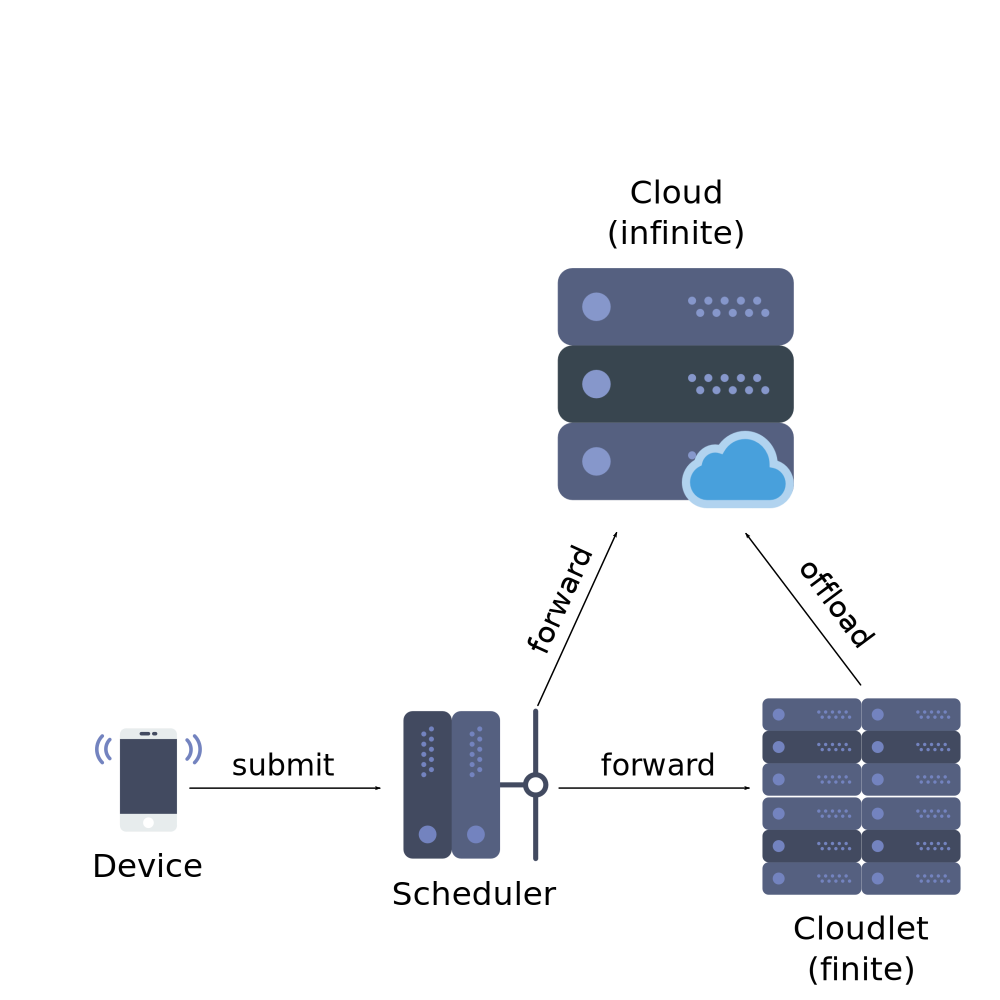
\includegraphics[width=\columnwidth]{fig/modeling-system-sketch}
	\caption{The system sketch.}
	\label{fig:modeling-system-sketch}
\end{figure}

We assume that
(i) the Cloudlet provides tasks with higher service rate than the Cloud, 
(ii) when a task is interrupted in the Cloudlet and it is sent to the Cloud, the restart process comes with a \textit{setup time overhead}.

% %
% GOALS AND OBJECTIVES
% %
\subsection{Goals and Objectives}
The main goals of simulation are about system tuning.
In particular, we propose to determine with a $95\%$ level of confidence
\begin{itemize}
	\item the response time as a function of the threshold $S$,
	\item the throughput as a function of the threshold $S$,
	\item the distribution of the response time when $S=N$ and
	\item the threshold of the off-loading policy that minimizes the response time.
\end{itemize}


% %
% CONCEPTUAL MODEL
% %
\subsection{Conceptual Model}
The conceptual model is depicted in Figure~\ref{fig:modeling-conceptual-model}.

\begin{figure}
	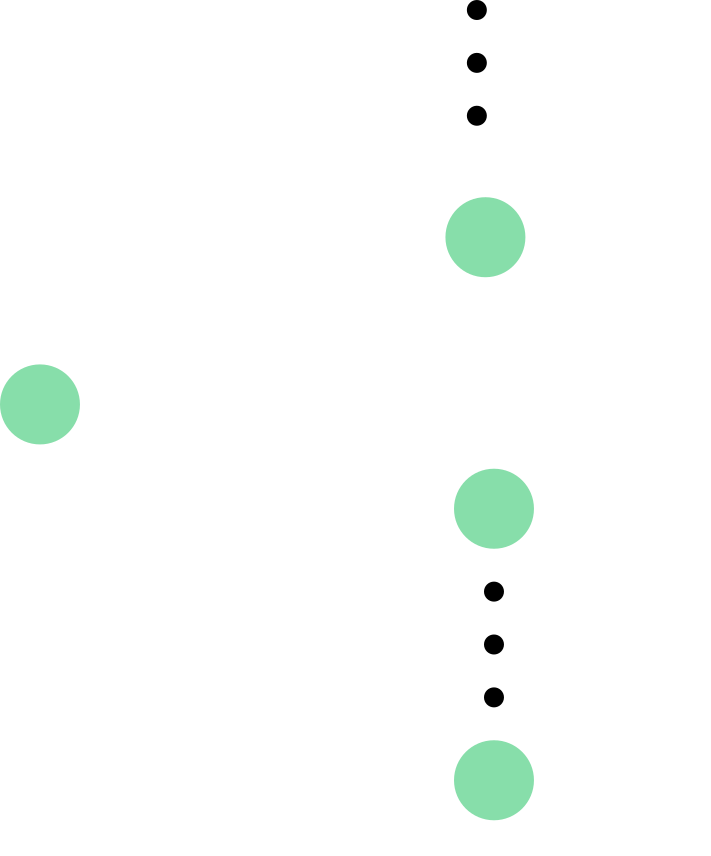
\includegraphics[width=\columnwidth]{fig/modeling-conceptual-model}
	\caption{The conceptual model.}
	\label{fig:modeling-conceptual-model}
\end{figure}

% %
% SPECIFICATION MODEL
% %
\subsection{Specification Model}
The state of a system is a comprehensive characterization of the system at a particular time.
The state of the system is represented by the pair $(n_{clt,1},n_{clt,2},n_{cld,1},n_{cld,2})$, where $n_{cld,i}$ is the number of tasks belonging to the $i$-th class within the Cloudlet and $n_{cld,i}$ is the number of tasks belonging to the $i$-th class within the Cloud.
An event is an occurrence that could change the state of the system at the event time, according to the event type.
Our events are ...

Tasks belonging to the first class, i.e. $t\in C_{1}$ arrive to the system with an exponential arrival process with rate $ \lambda_{1}$; whilst tasks belonging to the seconds class, i.e. $t\in C_{2}$ arrive to the system with an exponential arrival process with rate $ \lambda_{2}$.
The Cloudlet serves tasks belonging to the first class with exponentially distributed service time with rate $\mu_{cld,1}$; whilst the Cloudlet serves tasks belonging to the second class with exponentially distributed service time with rate $\mu_{cld,2}$.
The Cloud serves tasks belonging to the first class with exponentially distributed service time with rate $\mu_{clt,1}$; whilst the Cloudlet serves tasks belonging to the second class with exponentially distributed service time with rate $\mu_{clt,2}$.
We assume that 
(i) $\mu_{clt,i}>\mu_{cld,i}\ \forall i=1,2$ and
(ii) the setup time $T_{setup}$ is exponentially distributed with expected value $E[T_{setup}]$.

\begin{algorithm}
	\SetAlgoLined
	\If{task of class 1}{
		\If{$n_{clt}=N$}{
			send to Cloud
		} 
		\If{$n_{clt}+n_{cld}<S$}{
			accept
		} 
		\eIf{$n_{cld} > 0$}{
			accept on Cloudlet and send a class 2 task to Cloud
		}{
		accept on Cloudlet
		}
	}
	\If{arrival of class 2}{
		\eIf{$n_{clt}+n_{cld}>=S$}{
			send to Cloud
		}{
		accept on Cloudlet
	}
	}
	\caption{The offloading policy.}
	\label{alg:modeling-offloading-policy}
\end{algorithm}

% %
% COMPUTATIONAL MODEL
% %
\subsection{Computational Model}
The proposed performance model has been implemented as a Python application. 
The simulation parameters can be configured with a YAML file loaded by the simulator when it starts up.
The full open source code is available in a public repository \cite{gmarciani-pydes} and representative examples of configuration and outputs are presented in Section~\ref{sec:usage}.

We adopted the next-event simulation paradigm, using 
(i) a custom multi-stream Lehmer generator to generate random events, whose parameters have been described in Section~\ref{sec:random-number-generation} and whose evaluation is presented in Section~\ref{sec:evaluation}; and
(ii) a priority-queue based calendar with the ability both to schedule and un-schedule events.

Even if both the initial and terminal state can have any possible value, we adopted the convention of initializing and terminating the system in the idle state $(0,0,0,0)$. In particular, the terminal state is reached via the well-known closed door technique driven by a stop time condition.

The calendar is initialized by scheduling the first arrival in the initialization phase. The submission of an arrival $a$ to the system could induce
(i) the scheduling of the corresponding completion event,
(ii) the scheduling of a new arrival, or
(iii) the unscheduling of a previously scheduled completion, i.e. interruption in Cloudlet.

The next-event calendar is implemented as priority queue, appropriately extended to manage scheduling/unscheduling of events and exclusion of impossible events, i.e. arrivals with occurrence time greater than the stop time.
The impossibility of events is managed by letting the calendar contain possible events only, which is the best approach when the event list is assumed to be very long.


% %
% VERIFICATION
% %
\subsection{Verification}
The main goal of verification is to assess the consistency of the computational model with the specification model.
The verification has been carried out by evaluating the following consistency checks based on simulator logs and outputs:

\begin{itemize}
	\item \textbf{state consistency:} verifies the correctness of the system state evolution, i.e. state transitions;
	
	\item \textbf{arrival consistency:} verifies the correctness of arrivals ordering, i.e. tasks arrived before are served before;
	
	\item \textbf{service consistency:} verifies the correctness of service ordering, i.e. tasks with less service time leave the system before;
	
	\item \textbf{flow consistency:} verifies the correctness of flow trends, such as:
	
	\begin{equation}
	n_{clt,i}=a_{clt,i}-s_{clt,i}-c_{clt,i}
	\end{equation}
	\begin{equation}
	n_{cld,i}=a_{cld,i}+s_{cld,i}-c_{cld,i}
	\end{equation}
	\begin{equation}
	s_{clt,i}=s_{cld,i}
	\end{equation}
	
	where 
	$n_{j,i}$ is the population in the $j$-th subsystem belonging to $i$-th class of tasks, 
	$a_{j,i}$ is the number of arrivals to the $j$-th subsystem belonging to $i$-th class of tasks,
	$c_{j,i}$ is the number of completions in the $j$-th subsystem belonging to $i$-th class of tasks
	$s_{j,i}$ is the number of switches from/to the $j$-th subsystem belonging to $i$-th class of tasks\footnote{notice that $s_{j,1}=0\forall j=1,2$, as tasks belonging to class $C1$ cannot be switched from Cloudlet to Cloud.}.
	 
	\item \textbf{workload change consistency:} verifies the correctness of performance metrics variations in response to arrival/service rates variations. For example, we verified that the following hold true:
	
	\begin{equation}
		\mu_{cld,2}^{new} > \mu_{cld,2}^{old} \Rightarrow E[T_{sys,2}]^{new} > E[T_{sys,2}]^{old}
	\end{equation}
	\\
	and
	
	\begin{equation}
	S^{new} > S^{old} \Rightarrow E[N_{cld,2}]^{new} < E[N_{cld,2}]^{old}
	\end{equation}
\end{itemize}

% %
% VALIDATION
% %
\subsection{Validation}
It is well-known that model development should include a final validation step in order to assess the consistency of the model with the real system. 
%
As the simulation main purpose is insight, a widely adopted Turing-like technique is to place the computational model alongside with the real system and assess the consistency of performance indices.
%
Clearly, we cannot adopt this technique as we cannot compare the model with its real counterpart.
%
For this reason, we totally rely on the validation with respect to the analytical model. 
In Figure \ref{tbl:validation} we show the comparison between theoretical performance results, taken from the analytical model, and their experimental counterpart, taken from the simulator. 
The obtained results demonstrate that our simulator is a reliable tool to conduct the performance analysis of the target system.

\begin{figure}
	\begin{center}
		\begin{tabular}{|c||c|c|}
			\hline
			Index & Theoretical & Experimental\\
			\hline
			$E[N_{clt}]$  & $123456789$ & $123456789$ \\
			$E[N_{1,clt}]$  & $123456789$ & $123456789$ \\
			$E[N_{2,clt}]$  & $123456789$ & $123456789$ \\
			$E[T_{clt}]$  & $123456789$ & $123456789$ \\
			$E[T_{1,clt}]$  & $123456789$ & $123456789$ \\
			$E[T_{2,clt}]$  & $123456789$ & $123456789$ \\
			$X_{clt}$  & $123456789$ & $123456789$ \\
			$X_{1,clt}$  & $123456789$ & $123456789$ \\
			$X_{2,clt}$  & $123456789$ & $123456789$ \\
			\hline
			$E[N_{cld}]$  & $123456789$ & $123456789$ \\
			$E[N_{1,cld}]$  & $123456789$ & $123456789$ \\
			$E[N_{2,cld}]$  & $123456789$ & $123456789$ \\
			$E[T_{cld}]$  & $123456789$ & $123456789$ \\
			$E[T_{1,cld}]$  & $123456789$ & $123456789$ \\
			$E[T_{2,cld}]$  & $123456789$ & $123456789$ \\
			$X_{cld}$  & $123456789$ & $123456789$ \\
			$X_{1,cld}$  & $123456789$ & $123456789$ \\
			$X_{2,cld}$  & $123456789$ & $123456789$ \\
			\hline
			$E[N_{sys}]$  & $123456789$ & $123456789$ \\
			$E[N_{1,sys}]$  & $123456789$ & $123456789$ \\
			$E[N_{2,sys}]$  & $123456789$ & $123456789$ \\
			$E[T_{sys}]$  & $123456789$ & $123456789$ \\
			$E[T_{1,sys}]$  & $123456789$ & $123456789$ \\
			$E[T_{2,sys}]$  & $123456789$ & $123456789$ \\
			$X_{sys}$  & $123456789$ & $123456789$ \\
			$X_{1,sys}$  & $123456789$ & $123456789$ \\
			$X_{2,sys}$  & $123456789$ & $123456789$ \\
			\hline
		\end{tabular}
	\end{center}
	\caption{Validation: comparison between analytical results and experimental results.}
	\label{tbl:validation}
\end{figure}